\documentclass[11pt]{article}

\usepackage[T1]{fontenc}
\usepackage[polish]{babel}
\usepackage[utf8]{inputenc}
\usepackage{listings}
\usepackage{xcolor}
\usepackage{indentfirst}
\usepackage{graphicx}

\graphicspath{ {../plots/} }

\topmargin=-0.45in
\evensidemargin=0in
\oddsidemargin=0in
\textwidth=6.5in
\textheight=9.0in
\headsep=0.25in

\definecolor{codegreen}{rgb}{0,0.6,0}
\definecolor{codegray}{rgb}{0.5,0.5,0.5}
\definecolor{codepurple}{rgb}{0.58,0,0.82}
\definecolor{backcolour}{HTML}{F2F2F2}

\lstdefinestyle{mystyle}{
    backgroundcolor=\color{backcolour},   
    commentstyle=\color{codegreen},
    keywordstyle=\color{magenta},
    numberstyle=\tiny\color{codegray},
    stringstyle=\color{codepurple},
    basicstyle=\ttfamily\footnotesize,
    breakatwhitespace=false,         
    breaklines=true,                 
    captionpos=b,                    
    keepspaces=true,                 
    numbers=left,                    
    numbersep=5pt,                  
    showspaces=false,                
    showstringspaces=false,
    showtabs=false,                  
    tabsize=4
}

\lstset{style=mystyle}

\title{Projekt 2 WdAD}
\author{Filip Cebula 151410}
\date{\today}

\begin{document}

\maketitle
\pagebreak

\section{Zadanie 1}
\subsection{Model regresji}
Tworzymy model regresji w R, używając polecenia \textbf{lm()} i sprawdzamy
jego parametry korzystając z polecenia \textbf{summary}. Na potrzebę zadania
analizie poddamy zestaw danych \textit{crabs} z biblioteki MASS, który
zawiera informacje o rozmiarach badanych krabów.

\begin{lstlisting}[language=R]
regression = lm(CW ~ CL, data = crabs);
cat("\nRegression model width~length of crabs body\n");
summary(regression);
cat("\n");

# OUTPUT:
# Regression model width~length of crabs body
# 
# Call:
# lm(formula = CW ~ CL, data = crabs)
# 
# Residuals:
    # Min      1Q  Median      3Q     Max 
# -1.7683 -0.6088  0.1075  0.5394  1.8092 
# 
# Coefficients:
            # Estimate Std. Error t value Pr(>|t|)    
# (Intercept) 1.089919   0.257490   4.233 3.53e-05 ***
# CL          1.100266   0.007831 140.504  < 2e-16 ***
# Signif. codes:  0 '***' 0.001 '**' 0.01 '*' 0.05 '.' 0.1 ' ' 1
# 
# Residual standard error: 0.7864 on 198 degrees of freedom
# Multiple R-squared:  0.9901,	Adjusted R-squared:   0.99 
# F-statistic: 1.974e+04 on 1 and 198 DF,  p-value: < 2.2e-16
\end{lstlisting}


\subsection{Wykresy}
Generujemy wykresy do zadania, które pozwolą nam na lepszą analizę naszego
modelu.

\begin{lstlisting}[language=R]
png(file = "plots/scatterplot.png", height=1000, width=1000, res=150);
plot(x=crabs$CL, y=crabs$CW, xlab="Carapace length [mm]",
  ylab="Carapace width [mm]", main="Crab's carapace size");
abline(reg = regression, col = "red");
dev.off();

png(file = "plots/model_plots.png", height=1000, width=1000, res=150);
par(mfrow = c(2,2));
plot(regression);
dev.off();
\end{lstlisting}

\pagebreak

\subsection{Scatterplot}
\begin{figure}[h]
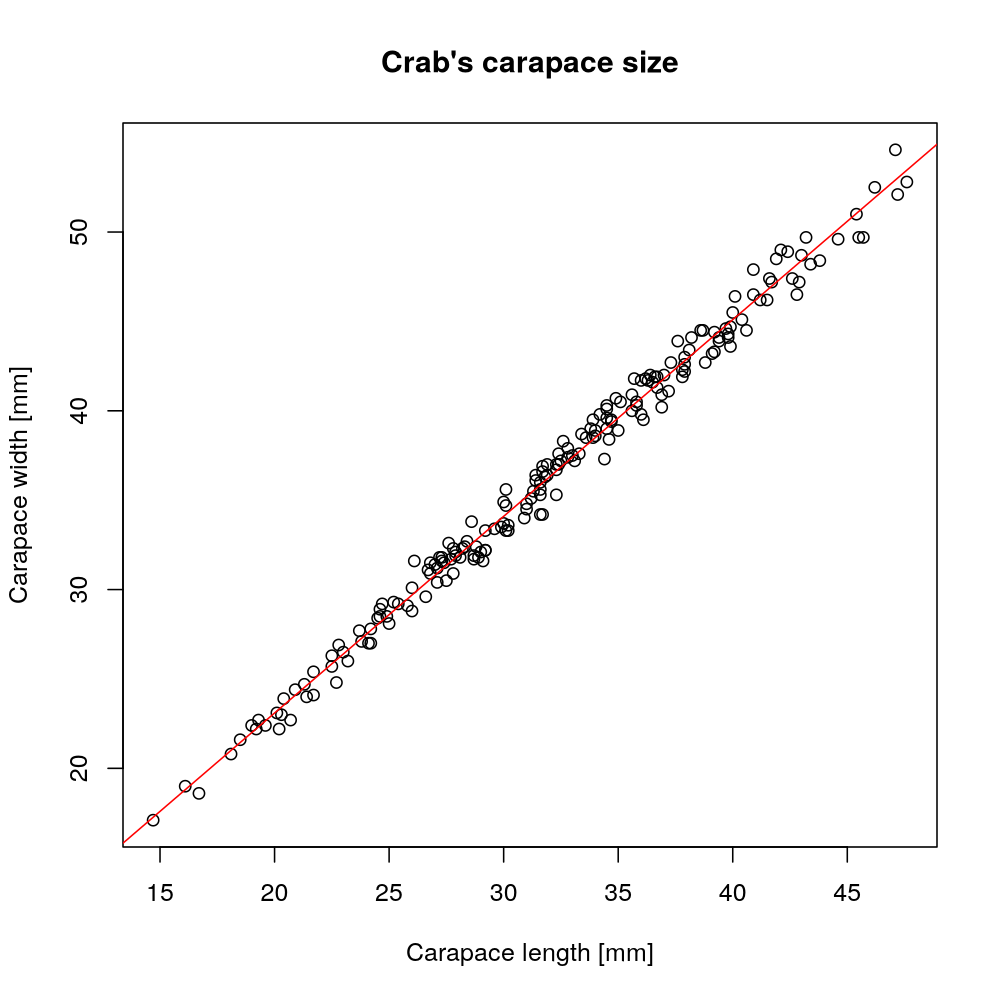
\includegraphics[scale=0.5]{scatterplot.png}
\centering
\end{figure}

\subsection{Wykresy diagnostyczne}
\begin{figure}[h]
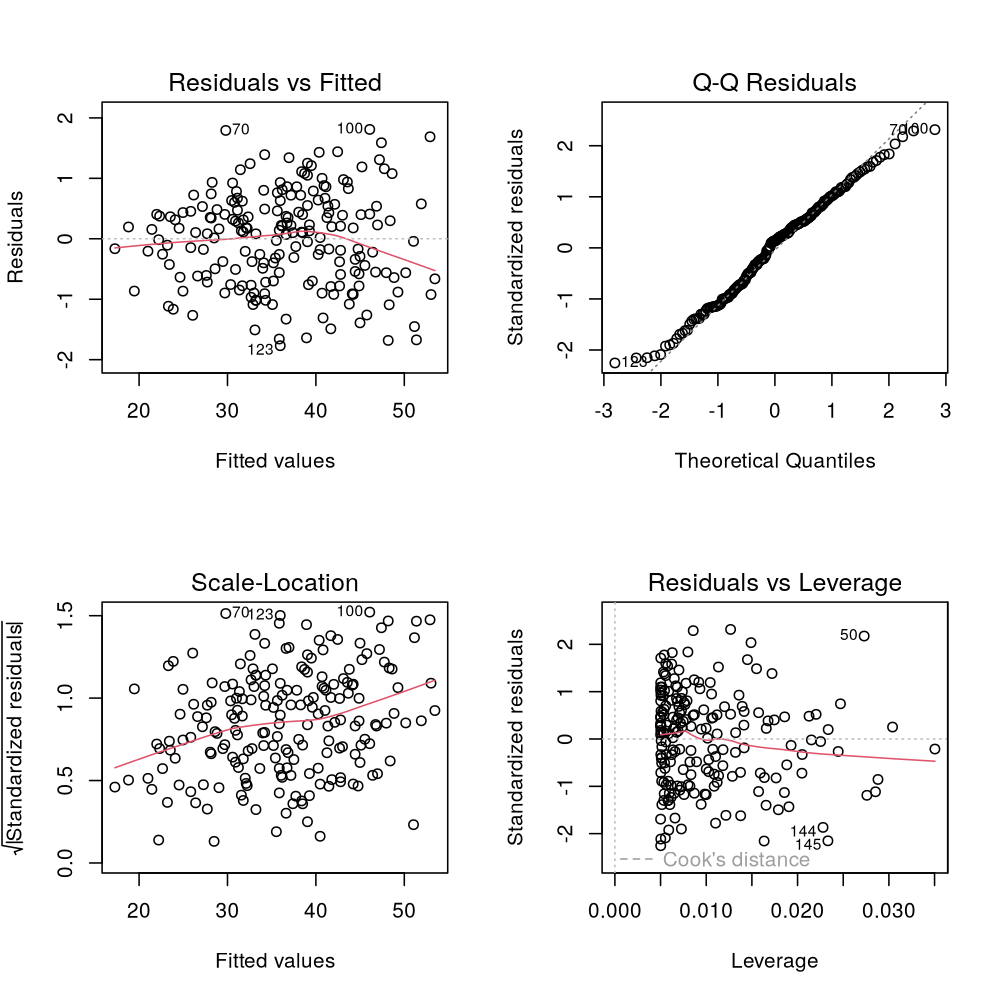
\includegraphics[scale=0.5]{model_plots.png}
\centering
\end{figure}

\pagebreak

\subsection{Wnioski}
Patrząc na wartość R-squared możemy wywnioskować, że nasz model wyjaśnia
99\% zmienności szerokości ciała kraba na podstawie jego długości. Sugeruje to,
że długość ciała ma silny wpływ na jego szerokość.

Widzimy że wszyskie residuals, mieszczą się w przedziale [-2;2], co oznacza,
że wartości faktyczne są bardzo mało oddalone od wartości, które przewiduje nasz
model.

Na podstawie wartości F-statistic i p-value, możemy odrzucić hipotezę zerową,
że nie ma relacji pomiędzy szerokością a długością ciała kraba.

Patrząc na scatterplot widzimy, że wszystkie punkty są blisko czerwonej lini
(lini przewidywanej przez nasz model) i nie ma wartości odstających, co sugeruje
że model jest dobrze dopasowany.

Z wykresu Residuals vs Fitted, możemy odczytać że liniowość jest zachowana
(patrząc na czerwoną linię), nie ma dużych wartości odstających (wszystkie są
w miarę zgrupowane), oraz że nasze wartości są homoskedastyczne (tzn. mają
podobną wariancje). Wykres Scale-Location potwierdza homoskedastyczność, którą
ustaliliśmy wcześniej.

Z wykresu kwantyl-kwantyl widzimy, że nasze wartości mają rozkład podobny do
normalnego, co wskazuje, że założenie o normalności reszt jest spełnione i nasz
model może być odpowiedni. Możemy jednak zwrócić uwagę na lekko długie ogony
naszego rozkładu, ale ich odchylenie od lini prostej wykresu jest stosunkowo
małe i występuje dla bardzo małej ilości wartości.

Z wykresu Residuals vs Leverage widzimy, że rozpiętość wartości na wykresie
jest stosunkowo równa i żadna wartość nie przekracza dystansu Cook'a, przez co
możemy stwierdzić, że nasz model nie ma dużo wartości odstających.

Na podstawie powyższych obserwacji możemy stwierdzić, że nasz model regresji
liniowej jest dobrze dopasowany do danych.

\pagebreak

\section{Zadanie 2}
\subsection{Współczynniki regresji}
Zakładamy, że mamy n obserwacji $(x_i,y_i)$, gdzie $i=1,2,\ldots,n$. Wiemy
także, że model regresji liniowej ma postać $y_i=b_0 + b_1 x_i$

Chcemy wyznaczyć $b_0$ i $b_1$, które minimalizują sumę kwadratów reszt. W tym
celu zapiszmy sumę kwadratów reszt jako funkcje dwóch zmiennych $b_0$ i $b_1$.

\begin{equation}
  X(b_0,b_1) = \sum_{i=1}^{n} (y_i - (b_0 + b_1 x_i))^2
\end{equation}

Aby znaleźć minima naszej funkcji za względu na parametry $b_0$ i $b_1$,
różniczkujemy ją po $b_0$ i $b_1$ i przyrównujemy do 0.

Dla $b_0$:

\begin{equation}
  \frac{\partial X}{\partial b_0} = \sum_{i=1}^{n} -2(y_i - (b_0 + b_i x_i)) = 0
\end{equation}

Co po uproszczeniu da nam:
\begin{equation}
  \sum_{i=1}^{n} y_i = nb_0 + b_1 \sum_{i=1}^{n} x_i
\end{equation}

Dla $b_1$:
\begin{equation}
  \frac{\partial X}{\partial b_1} = \sum_{i=1}^{n} -2x_i(y_i - (b_0 + b_i x_i)) = 0
\end{equation}

Co po uproszczeniu da nam:
\begin{equation}
  \sum_{i=1}^{n} x_i y_i = b_0 \sum_{i=1}^{n} x_i + b_1 \sum_{i=1}^{n} x_i^2
\end{equation}

Wyliczamy $b_0$ korzystając ze wzoru na średnią ($\overline{x} = \frac{1}{n} \sum_{i=0}^{n}$):
\begin{equation}
  n \overline{y} = n b_0 + n \overline{x} b_1 \Rightarrow b_0 = \overline{y} - \overline{x} b_1
\end{equation}

Wyliczamy $b_1$ korzystając ze wzory na średnią oraz wyliczonego wcześniej przez
nas $b_0$
\begin{equation}
  \sum_{i=1}^{n} x_i y_i = (\overline{y} - \overline{x} b_1) \sum_{i=1}^{n} x_i + b_1 \sum_{i=1}^{n} x_i^2 \Rightarrow \sum_{i=1}^{n} x_i y_i = n\overline{x}\overline{y} - b_1 n \overline{x}^2 + b_1 \sum_{i=1}^{n} x_i^2
\end{equation}

Otrzymujemy więc:
\begin{equation}
b_0 = \overline{y} - \overline{x} b_1
\end{equation}
\begin{equation}
  b_1 = \frac{\sum_{i=1}^{n} x_i y_i - n\overline{x}\overline{y}}{\sum_{i=1}^{n} x_i^2 - n \overline{x}^2}
\end{equation}

\pagebreak

\subsection{Dowód 1}
Rozwijamy lewą stronę:
\begin{equation}
  \sum_{i=1}^{n}(x_i^2 - 2x_i\overline{x} + \overline{x}^2) = \sum_{i=1}^{n} x_i^2 - 2\overline{x}\sum_{i=1}^{n} + n\overline{x}^2
\end{equation}

Ze wzoru na średnią:
\begin{equation}
  \sum_{i=1}^{n}x_i^2 - 2n\overline{x}^2 + n\overline{x}^2 = \sum_{i=1}^{n} x_i^2 - n\overline{x}^2
  = \sum_{i=1}^{n} x_i^2 - \frac{1}{n} (\sum_{i=1}^{n} x_i)^2
\end{equation}

Co kończy dowód.

\subsection{Dowód 2}

\subsection{Wzór na współczynnik $b_1$}

\end{document}
